\section{Verlustbehaftete Kompression von volumetrischen Punkten}
Moderne Simulationen sind in der Lage grosse Mengen an Daten zu produzieren. Die rohe Datenmenge ist oft zu gross um sie zu archivieren oder in vernünftiger Zeit über eine Internetverbindung zu übertragen. In wissenschaftlichen Anwendungen können natürliche Phänomene wie Schwingungen, Flugbahnen, Kraftfelder etc. als Linien im dreidimensionalen Raum abgebildet werden. Eine wissenschaftliche Simulation erstellt eine Menge an volumetrischen Punkten, welche die Linien im Raum darstellen. Ziel dieser Arbeit ist es eine verlustbehaftete Kompression von wissenschaftlichen Daten zu entwickeln, welche die Übertragung über eine Internetverbindung ermöglicht.\\
[\baselineskip]
Im Rahmen dieses Projekts sollen Daten von Magnetfeldlinien der Sonne komprimiert werden, welche über eine Internetverbindung zum JHelioviewer übertragen werden. Der JHelioviewer ist eine Applikation zur visualisierung von Satellitenmessdaten und Simulationen der Sonne. Die Applikation wird von der ESA und der FHNW entwickelt. Die Abbildung \ref{einleitung::feldlinien} zeigt eine Visualisierung des JHelioviewers von der Sonnenoberfläche und Feldlinien.\\
\begin{figure}[!htbp]
\center
	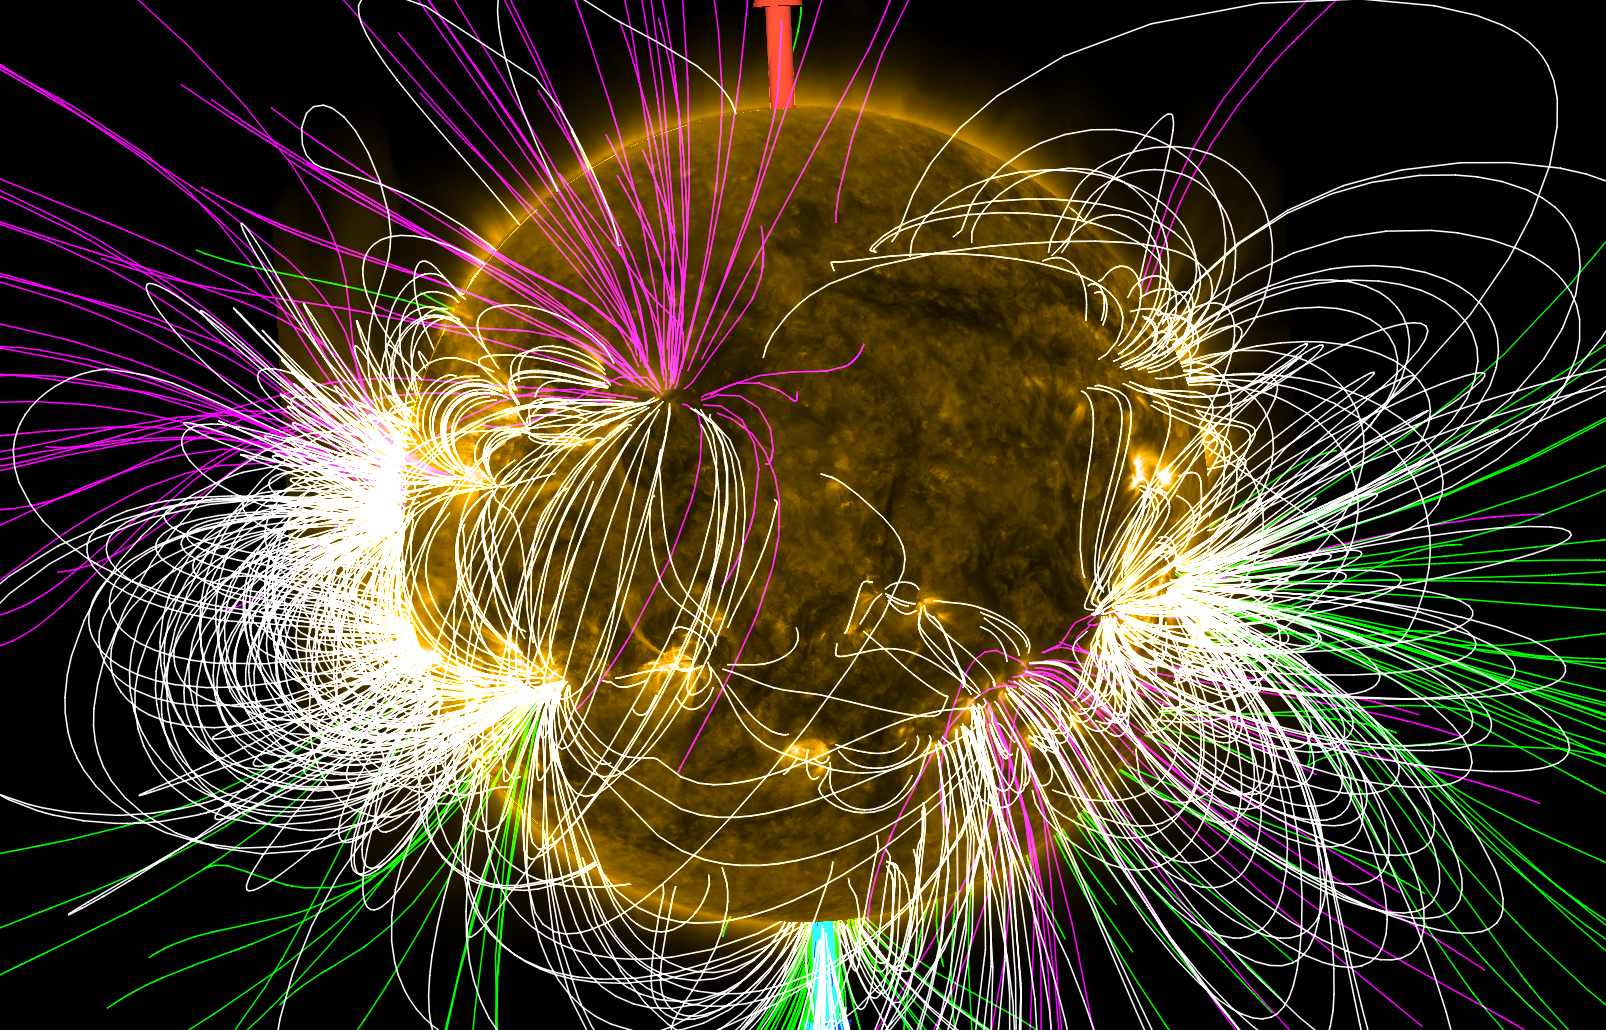
\includegraphics[width=0.8\textwidth,height=8cm,keepaspectratio]{./pictures/einleitung/fieldLines.png}
	\caption{Visualisierung der Feldlinien im JHelioviewer}
	\label{einleitung::feldlinien}
\end{figure}
Auf der Visualisierung sind Feldlinien in drei unterschiedlichen Farben zu erkennen, welche drei unterschiedle Typen darstellen: Linien, die auf der Sonne starten und wieder auf der Sonne landen, auf der Sonne starten und ins Weltall führen oder vom Weltall auf der Sonne landen. Die weissen Feldlinien repräsentieren ''Sonne zu Sonne´´, die Grünen ''Sonne zu Weltall´´ und die Violetten ''Weltall zu Sonne´´.\\
[\baselineskip]
Der JHelioviewer visualisiert mehrere Messungen oder Simulationen in Abfolge. Ziel ist es, möglichst schnell die Mess- und Simulationsdaten abzuspielen, sodass der Benutzer eine flüssige Animation erhält. Pro Simulation werden etwa 1.5 MiByte and Feldliniendaten generiert. Bei einer Visualisierung muss der JHelioviewer die Feldlinien- und andere Daten zur Laufzeit herunterladen, was hohe Anforderungen an die  Internetverbindung stellt.
Internetverbindung wird stark beansprucht und Benutzer muss auf Frames warten.

Potential Field Source Surface (PFSS) Simulation, welche aus Messungen der Sonnenoberfläche die Magnetfeldlinien extrapoliert, produziert pro Aufnahme etwa 1.5 Mibyte an Daten. welche zur Laufzeit über eine Internetverbindung heruntergeladen wird. Mit einer verlustbehafteten Kompression soll die zu übertragende Datenmenge deutlich verkleinert werden.

Resultate

Wo was beschrieben wird.